%%%%%%%%%%%%%%%%%%%%%%%%%%%%%%%%%%%%%%%%%%%%%%%%%%%%%%%%%%%%%%%%%%%%%%%%%%%%%%%
\section{Task parallelism}
%%%%%%%%%%%%%%%%%%%%%%%%%%%%%%%%%%%%%%%%%%%%%%%%%%%%%%%%%%%%%%%%%%%%%%%%%%%%%%%
%%%%%%%%%%%%%%%%%%%%%%%%%%%%%%%%%%%%%%%%%%%%%%%%%%%%%%%%%%%%%%%%%%%%%%%%%%%%%%%
\subsection{Task parallelism}
%------------------------------------------------------------------------------
\begin{frame}
  \frametitle{Task parallelism}
  \begin{block}{Task parallelism}
    \begin{itemize}
    \item {\bf Task parallelism} or \blue{functional parallelism} or \blue{control parallelism}.
    \item Decomposes the \red{computation} rather than the \red{manipulated data}.
      \begin{itemize}
      \item Programming model for tasks that perform different computations.
      \end{itemize}
    \item Ex.: Cilk, Intel TBB, OpenMP.
    \end{itemize}
  \end{block}
  %
  \pause
  %
  \begin{exampleblock}{Task dependency}
    \begin{itemize}
    \item Tasks with dependencies can unfold a \red{directed acyclic graph} (DAG).
      \begin{itemize}
      \item Expressed by synchronization such as \texttt{sync} keyword.
      \end{itemize}
    \item If data dependencies are considered, the algorithm unfolds a \red{data flow graph} (DFG).
    \item Ex.: Jade, Athapascan, OpenMP (\red{new}), KAAPI/XKaapi, StarPU, OmpSs, 
      Intel Offload.
    \end{itemize}
  \end{exampleblock}
\end{frame}
%------------------------------------------------------------------------------
%%%%%%%%%%%%%%%%%%%%%%%%%%%%%%%%%%%%%%%%%%%%%%%%%%%%%%%%%%%%%%%%%%%%%%%%%%%%%%%
%% \subsection{Intel Cilk Plus}
%% %------------------------------------------------------------------------------
%% \begin{frame}[fragile]
%%   \frametitle{Intel Cilk Plus}
%%   \begin{itemize}
%%   \item Extensions to C/C++ to support {\bf fork-join parallelism}.
%%     \begin{itemize}
%%     \item Based on Cilk (MIT) and Cilk++ (Cilk Arts).
%%     \end{itemize}
%%   \item Efficient work-stealing scheduler.
%%   \item Offers \blue{hyperobjects} (lock-free mechanism).
%%   \end{itemize}
%%   %
%%   \begin{exampleblock}{Cilk Plus keywords}
%%     \begin{itemize}
%%     \item \verb+cilk_spawn+ - asynchronous function call.
%%     \item \verb+cilk_sync+ - synchronization, must wait all spawned tasks.
%%     \item \verb+cilk_for+ - parallel iterations.
%%     \end{itemize}
%%   \end{exampleblock}
%% \end{frame}
%% %------------------------------------------------------------------------------
%% \begin{frame}[fragile]
%%   \frametitle{Intel Cilk Plus}
%%   \vspace{-4mm}
%%   \begin{columns}
%%     \begin{column}{0.5\textwidth}
%%   \begin{block}{Thread parallelism}
%% \begin{lstlisting}
%% main(void)
%% {
%%   cilk_spawn f();
%%   cilk_spawn g();
%%   // nop
%%   cilk_sync;
%% }
%% \end{lstlisting}
%%   \end{block}
%%     \end{column}
%%     %
%%     \begin{column}{0.5\textwidth}
%%       \begin{flushleft}
%% 	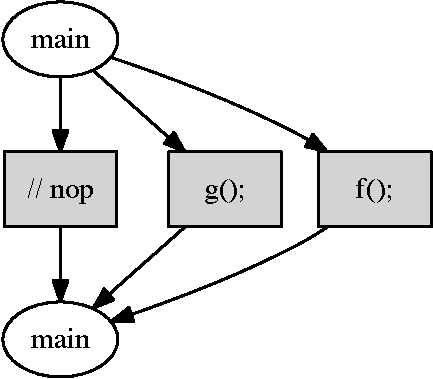
\includegraphics[width=\textwidth]{cilk-fork-1-crop}
%%       \end{flushleft}
%%     \end{column}
%%   \end{columns}
%% \end{frame}
%% %------------------------------------------------------------------------------
%% \begin{frame}[fragile]
%%   \frametitle{Intel Cilk Plus}
%%   \vspace{-4mm}
%%   \begin{columns}
%%     \begin{column}{0.5\textwidth}
%%   \begin{block}{Thread parallelism}
%% \begin{lstlisting}
%% main(void) 
%% {
%%   cilk_spawn f();
%%   g();
%%   // nop
%%   cilk_sync;
%% }
%% \end{lstlisting}
%%   \end{block}
%%     \end{column}
%%     %
%%     \begin{column}{0.5\textwidth}
%%       \begin{flushleft}
%% 	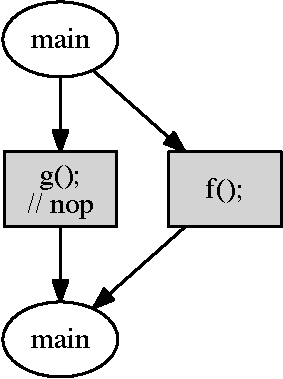
\includegraphics[width=0.7\textwidth]{cilk-fork-2-crop}
%%       \end{flushleft}
%%     \end{column}
%%   \end{columns}
%% \end{frame}
%% %------------------------------------------------------------------------------
%% \begin{frame}[fragile]
%%   \frametitle{Intel Cilk Plus}
%%   \begin{block}{Parallel loops}
%% \begin{lstlisting}
%% for( int i = 0; i < n; i++ )
%% {
%%   cilk_spawn do_work(i);
%% }
%% cilk_sync;
%% \end{lstlisting}
%%   \end{block}
%%   %
%%   \pause
%%   %
%%   \begin{exampleblock}{Parallel loops (divide-and-conquer)}
%% \begin{lstlisting}
%% cilk_for for( int i = 0; i < n; i++ )
%% {
%%   do_work(i);
%% }
%% \end{lstlisting}
%%   \end{exampleblock}
%% \end{frame}
%% %------------------------------------------------------------------------------
%% %%%%%%%%%%%%%%%%%%%%%%%%%%%%%%%%%%%%%%%%%%%%%%%%%%%%%%%%%%%%%%%%%%%%%%%%%%%%%%%
%% %\subsection{Intel TBB}
%% %------------------------------------------------------------------------------
%% %\begin{frame}
%% %  \frametitle{Intel Threading Building Blocks}
%% %\end{frame}
%------------------------------------------------------------------------------
%%%%%%%%%%%%%%%%%%%%%%%%%%%%%%%%%%%%%%%%%%%%%%%%%%%%%%%%%%%%%%%%%%%%%%%%%%%%%%%
\subsection{OpenMP}
%------------------------------------------------------------------------------
\begin{frame}[fragile]
  \frametitle{OpenMP tasks}
\begin{block}{Task construct}
\begin{lstlisting}
#pragma omp task
\end{lstlisting}
\end{block}
%
\pause
%
\begin{block}{Barrier \texttt{taskwait}}
\begin{lstlisting}
#pragma omp taskwait
\end{lstlisting}
\end{block}
%
\pause
%
\begin{itemize}
\item Independent units of work.
\item Recursive tasks.
\item Unfold parallelism at runtime.
\item The OpenMP implementation decides when/where to execute: 
  \begin{itemize}
  \item Immediately (in depth, \blue{depth-first} or \blue{work-first})
  \item Latter (in breadth, \blue{breadth-first} or \blue{help-first})
  \end{itemize}
\end{itemize}
%
\end{frame}
%------------------------------------------------------------------------------
\begin{frame}[fragile]
  \frametitle{OpenMP tasks}
\begin{block}{Linked list}
\begin{lstlisting}
node* p = head;
while(p) {
  process(p);
  p = p->next;
}
\end{lstlisting}
\end{block}
%
\end{frame}
%------------------------------------------------------------------------------
% \begin{frame}[fragile]
%   \frametitle{OpenMP tasks}
% \begin{block}{Linked list - parallel version}
% \begin{lstlisting}
% #pragma omp parallel
% {
% #pragma omp single 
%   {
%     node* p = head;
%     while(p) {
% #pragma omp task 
%       process(p);
%       p = p->next;
%     }
%   }
% }
% \end{lstlisting}
% \end{block}
% %
% \end{frame}
%------------------------------------------------------------------------------
\begin{frame}[fragile]
  \frametitle{OpenMP tasks}
\begin{block}{Linked list - parallel version}
\begin{lstlisting}
#pragma omp parallel
{
#pragma omp single 
  {
    node* p = head;
    while(p) {
#pragma omp task firstprivate(p)
      process(p);
      p = p->next;
    }
  }
}
\end{lstlisting}
\end{block}
%
\end{frame}
%------------------------------------------------------------------------------
\begin{frame}[fragile]
  \frametitle{OpenMP tasks}
\begin{block}{Cálculo de Fibonacci}
\begin{lstlisting}
int fib( int n ) {
  int x, y;
  if( n < 2 ) return n;
  x = fib( n - 1);
  y = fib( n - 2);
  return x + y;
}
\end{lstlisting}
\end{block}
%
\end{frame}
%------------------------------------------------------------------------------
\begin{frame}[fragile]
  \frametitle{Paralelismo de Tarefas}
\begin{block}{Cálculo de Fibonacci com OpenMP}
\begin{lstlisting}
int fib( int n ) {
  int x, y;
  if( n < 2 ) return n;
#pragma omp task
  x = fib( n - 1);
#pragma omp task
  y = fib( n - 2);
#pragma omp taskwait
  return x + y;
}
\end{lstlisting}
\end{block}
%
\onslide<2->
%
\begin{alertblock}{Correto?}
\onslide<3->{Não pois x e y são privados fora do escopo das tarefas.}
\end{alertblock}
%
\end{frame}
%------------------------------------------------------------------------------
\begin{frame}[fragile]
  \frametitle{Paralelismo de Tarefas}
\begin{block}{Cálculo de Fibonacci com OpenMP}
\begin{lstlisting}
int fib( int n ) {
  int x, y;
  if( n < 2 ) return n;
#pragma omp task shared(x)
  x = fib( n - 1);
#pragma omp task shared(y)
  y = fib( n - 2);
#pragma omp taskwait
  return x + y;
}
\end{lstlisting}
\end{block}
%
\begin{exampleblock}{Agora sim}
Necessitamos dos dois valores no cálculo.
\end{exampleblock}
%
\end{frame}
%------------------------------------------------------------------------------
